\section{Měření indukčnosti}
Měření hodnoty indukčnosti se stává samostatnou částí a je provedeno, po všech ostatních měřeních, se všemi
nalezenými odpory s menšími než \(2100\Omega\).
Metoda měření je založena na principu, že při zavírání okruhu proud stoupá
podle vzorce \(Il~=~Imax~\cdot~(1~-~\exp{\frac{-t}{\tau}})\).
Časová konstanta \(\tau = \frac{L}{R}\) je úměrná indukčnosti~\(L\), ale naopak nepřímo
úměrná odporu~\(R\).
Proud může být měřen pouze nepřímo jako úbytek napětí na odporu.
Naneštěstí, vzhledem k relativně vysokému \(680\Omega\) odporu, se časová konstanta dále snižuje.
A také to, že to stěžuje měřit malé indukčnosti s \(8MHz\) taktem.
Pro určení časové konstanty se napětí na \(680\Omega\) odporu stává snímačem proudu a je kontrolováno
analogovým komparátorem.

Pokud je pokles napětí napříč \(680\Omega\) odporem větší než referenční napětí interního referenčního napětí,
hlásí to komparátor, na při startu měření spuštěného 16 bitového čítače, který tuto událost přidává.
Eventuální přetečení čítače program přičte.
Pokud je napětí větší, počítadlo se okamžitě zastaví a z naměřeného záznamu měřiče a přepočtu
přepadu je určen celkový čas.
Připojení cívky je opět přepnuto z VCC na GND a prostřednictvím monitorování napětí jsou oba porty obslouženy,
dokud není detekován žádný proud.
Schéma zapojení~\ref{fig:Inductance} ukazuje zjednodušený diagram situace měření.

\begin{figure}[H]
\centering
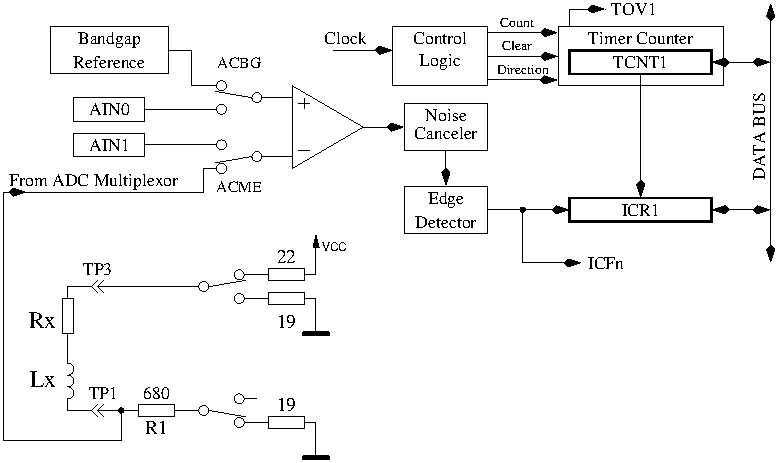
\includegraphics[width=.8\textwidth]{../FIG/Inductance.pdf}
\caption{Měření indukčnosti s komparátorem}
\label{fig:Inductance}
\end{figure}

Z napájecího napětí VCC a součtu všech odporů v obvodu, je možné maximální proud Imax a
z toho poměr referenčního napětí vzhledem k měření maximálního napětí na \(680\Omega\) odporu
\(Umax~=~Imax~\cdot~(680~+~19)\) určit.
Pomocí vzorce \(L~=~-\frac{t~\cdot~Rges}{\log{(1~-~\frac{Uref}{Umax})}}\) lze určit indukčnost.
Přirozený logaritmus je v programu určen tabulkou.
Rozlišení indukčnosti je pro tento typ měření nastaveno na hodnotu \(0,1mH\).
Abychom mohli měřit ještě menší indukčnosti, je v okruhu \(680\Omega\) odpor vynechán,
když byla měřena hodnota odporu cívky menší než \(24\Omega\).
Jako měřicí odpor pro měření proudu je v tomto případě použitý výstupní (\(19\Omega\)) odpor výstupních portů mcu. V tomto případě se špičkový proud stává větší než umožňuje specifikace ATmega.
Vzhledem k tomu, že se to děje jen velmi krátkou dobu, neočekávám žádné poruchy.
K vyloučení delšího časového období s nadměrným proudem, bude vždy provedeno dodatečné měření, pomocí
zpožděně spuštěného čítače přes \(680\Omega\) odpor.
Pro tento typ měření je rozlišení indukčnosti nastaveno na hodnotu \(0,01mH\).
Aby výsledky měření odpovídaly skutečné hodnotě indukčnosti, bude se od výsledku odečítat nulový ofset 6,
pokud je měřen bez \(680\Omega\). Jinak je odečtený nulový ofset 7 nebo 8.
U velkých indukčností mohou parazitní kapacity zvýšit proud tak rychle, že
monitorování napětí s komparátorem okamžitě reaguje.
K zajištění určení indukčnosti je stejné měření znovu provedeno, ale čítač je o něco později spuštěn,
aby bylo měřeno zvýšené napětí způsobené aktuálním zvýšením indukčnosti a nikoliv
špičkou přes parazitní kapacitu.
Měření probíhá v obou směrech. Ze dvou měření ve stejném směru proudění se používá vyšší výsledek měření.
Z měření v různých směrech proudu se používá menší hodnota jako výsledek měření indukčnosti.

\subsection{Výsledky měření indukčnosti}
Obrázek~\ref{fig:Induct328p} zobrazuje výsledky měření různých induktorů.

Indukčnosti nad \(1 H\) jsou relé a primární vinutí výkonových transformátorů, které je obtížné, kvůli
remanenci železného jádra vůbec měřit.

\begin{figure}[H]
\centering
\includegraphics[width=.8\textwidth]{../GNU/induct328pCZ.pdf}
\caption{Chyba měření indukčnosti 15 různých ATmega}
\label{fig:Induct328p}
\end{figure}

\subsection{Měření malých indukčností metodou vzorkování}

Nejmenší detekovatelná indukčnost při normální metodě měření je \(0,01mH\).
U vysokofrekvenčních aplikací má však měření menších hodnot indukčnosti smysl.
Normální měření používá pro stanovení indukčnosti aktuální nárůst proudu v cívce.
Tento způsob není použitelný pro metodu odběru vzorků, protože neexistují žádná měření pro metodu odběru vzorků
bez použití dalších odporů.
Proud tak rychle dosáhne nepřípustně vysoké hodnoty.
Poškození ATmegy je při normálním měření zabráněno pouze dřívějším vypnutím napájení.
Pro metodou výběru vzorku by bylo vypnutí obtížně proveditelné a kromě toho by kritický proces
musel být opakován mnohokrát za sebou.
Z tohoto důvodu používá holandský radioamatér Pieter-Tjerk (PA3FWM) jinou metodu pro toto měření.
S paralelně připojeným kondenzátorem k indukčností je vytvořený rezonanční obvod.
Krátkým proudovým impulzem je rezonanční obvod nabuzen a metoda vzorkování se pokouší určit
přirozenou frekvenci tohoto rezonančního obvodu.
Protože jeden konec cívky musí být udržován na potenciálu země pro měření ADC,
existují dva problémy. Samozřejmě jde vibrační napětí také do záporné oblasti.
Zde je oscilace přes interní ochrannou diodu ATmega omezené na přibližně \(0,6V\).
Tímto je také kladné špičkové napětí oscilace omezené na tuto hodnotu.
Kromě toho může ADC měřit pouze kladná napětí.
To je důvod, proč chybí negativní část oscilace. Namísto negativního napětí čte ADC vždy nulu.
Nicméně se Pieter-Tjerk podařilo, dostat přirozený kmitočet dostatečně přesný k určení naměřených dat ADC.
Z přirozené frekvence rezonančního obvodu může být, pokud je známa hodnota kapacity, vypočtena indukčnost.
Z tohoto důvodu je kalibrace rozšířena o měření paralelní kapacity pro měření indukčnosti.
Kondenzátor je požadován se zprávou ,,\mbox{\begin{large}1 \electricC 3~10-30nF(L)\end{large}}''.
Nekalibrovaný tester má výchozí hodnotu \(18nF\).
Hodnoty pro paralelní kondenzátor jsou relativně vysoko zvolené,
aby zůstal rezonanční obvod i při menších indukčnostech malý.
Kondenzátor pro paralelní připojení by měl mít vysokou kvalitu (typ fólie), vzhledem k tomu,
že kvalita rezonančního obvodu je určena z poklesu amplitudy napětí.
Při vysoké kvalitě kondenzátoru je obvykle cívka určující kvalitu rezonančního obvodu.
Pro obsluhu není nutná, kromě připojení paralelního kondenzátoru, žádná další akce.
Rezonanční obvod je pak detekován automaticky.
Pokud byl rezonanční obvod detekován, ukáže se za indukčností text ,,if'' a předpokládaná
kapacita paralelního kondenzátoru je uvedena v druhém řádku.
V tomto případě je také výstupní hodnota odporu cívky zobrazena na konci 1 řádku.
Hodnota odporu by měla být určitě kontrolována bez paralelně zapojeného kondenzátoru,
protože měření odporu na rezonančním obvodu často nefunguje!
V dalším řádku se uvádí měřená kmitočtová frekvence a kvalita Q.
Pokud nebyl žádný rezonanční obvod detekován, ukáže se odpor a indukčnost ve druhém řádku.
V příštím řádku je zobrazena rezonanční frekvence a kvalita, pokut je zjištěna,
i bez paralelního kondenzátoru, rezonance cívky.
Pro vzduchovou cívku se 6 závity a paralelně zapojený \(18nF\) kondenzátor 
určuje metoda odběru vzorků následující výsledek:

\begin{verbatim}
260nH if 18.1nF
2306kHz Q=38.7
\end{verbatim}

ATmega328 byl provozován s \(8MHz\).
Ke stejném výsledku se také dosáhlo s \(25cm\) dlouhým měděným drátem ohnutým do velkého kruhu.
Naměřená indukčnost je v tomto měření příliš vysoká, protože byl připojený vinutý svitkový
kondenzátor s vlastní indukčností.
V následující tabulce \ref{tab:littleInductors} jsou výsledky měření různých cívek,
které byly určeny s testerem a kmitočtovou frekvencí \(16MHz\).

\begin{table}[H]
\begin{center}
\begin{tabular}{| l | c | c | c | c | c |}
\hline
\hspace{1.5cm} Cp= & 6.68nF    & 11.4nF    & 18.2nF    & 20.3nF    & 33.3nF \\
Lp=           &           &           &           &           &        \\ 
\hline
\hline
3 turns, 13mm & 100nH     & 116nH     & 108nH     & 115nH     & 111nH  \\
 (91.4nH) & 6.039MHz  & 4.358MHz  & 3.568Mhz  & 3.282MHz  & 2.619MHz \\
              & Q=29.9    & Q=15.6    & Q=49.8    & Q=12.1    & Q=31.4  \\
\hline
4 turns, 13mm & 141nH     & 161nH     & 151nH     & 152nH     & 153nH  \\
 (144.9nH)     & 5.172MHz  & 3.724MHz  & 3.03Mhz   & 2.86MHz   & 2.226MHz \\
              & Q=44.8    & Q=16.0    & Q=46.2    & Q=14.6    & Q=30.5  \\
\hline
6 turns, 13mm & 217nH     & 232nH     & 223nH     & 224nH     & 227nH  \\
 (212.5nH)    & 4.18MHz   & 3.094MHz  & 2.492Mhz  & 2.343MHz  & 1.832MHz \\
              & Q=30.5    & Q=18.4    & Q=43.0    & Q=15.4    & Q=31.7  \\
\hline
12 turns, 13mm     & 547nH     & 571nH     & 559nH     & 560nH     & 566nH  \\
 (569.5nH)    & 2.632MHz  & 1.973MHz  & 1.573Mhz  & 1.491MHz  & 1.16MHz \\
              & Q=36.9    & Q=26.4    & Q=50.6    & Q=20.8    & Q=39.2  \\
\hline
27 turns, 11mm & \(1.93\mu H\) & \(1.92\mu H\) & \(2.02\mu H\) & \(2.00\mu H\) & \(2.01\mu H\)  \\
(\(1.9\mu H\)) & 1.403MHz  & 1.067MHz  & 828.5khz  & 789.5kHz  & 615.4kHz \\
              & Q=36.5    & Q=33.4    & Q=43.6    & Q=26.6    & Q=34.5  \\
\hline
\(6.3\mu H\)  & \(6.69\mu H\) & \(6.84\mu H\) & \(6.84\mu H\) & \(6.82\mu H\) & \(6.90\mu H\)  \\
\(7.12\mu H\) & 752.9kHz  & 570.2kHz  & 449.9khz  & 428.1kHz  & 332.3kHz \\
              & Q=28.5    & Q=30.5    & Q=32.3    & Q=25.5    & Q=28.3  \\
\hline
\end{tabular}
\end{center}
\caption{Výsledky měření některých malých cívek}
\label{tab:littleInductors}
\end{table}

Kondenzátory v této tabulce jsou vzorky s nízkou indukčností řady WIMA MKS.
Cívka se 4 závity ukazuje se svitkovým \(18.2nF\) paralelním kondenzátorem \(196nH\) indukčnost
namísto \(151nH\)  z tabulky.
S výjimkou posledního induktoru se jedná o samovolně vinuté cívky,
jejíž vypočtená indukčnost je uvedena v závorkách.
Poslední \(6.3\mu H\) cívka je průmyslově vyrobený vzorek označený \(6.3\mu H\).
Měření pomocí měřícího  RCL přístroje při \(100kHz\) má ale za výsledek indukčnost \(7.12\mu H\)!
Tabulka také ukazuje různé Q kvality pro stejnou cívku a téměř stejné paralelní kapacity.
Pro cívku s 12 závity je ukázána kvalita Q \(50.2\) s hodnotou \(18.2nF\) kondenzátoru,
ale s paralelní kapacitou \(20.3nF\) pouze \(20.8\).
To naznačuje podezření na chybu programu.
Pro kontrolu jsou na obrázku \ref{fig:W12compare} zobrazena data ADC převodníku pro
cívku s 12 závity a pro kondenzátory \(18.2nF\) a \(20.3nF\).
Dokonce i se surovými daty je jasný rozdíl pro obě varianty rezonančního obvodu rozpoznat.
Pravděpodobně je  příčinou rozdílu kvality typ použitého kondenzátoru.

\begin{figure}[H]
\centering
\includegraphics[width=.8\textwidth]{../GNU/W12compareCZ.pdf}
\caption{ ADC data ze dvou rezonančních obvodů s 12-závitovou cívkou}
\label{fig:W12compare}
\end{figure}

